\documentclass[11pt]{article}
\usepackage[utf8]{inputenc}
\usepackage[T1]{fontenc}
\usepackage[spanish]{babel}
\usepackage{amsmath, amssymb, amsthm}
\usepackage{braket}
\usepackage{graphicx}
\usepackage[margin=2.5cm]{geometry}
\usepackage{hyperref}

\allowdisplaybreaks

\newcommand{\ii}{\mathrm{i}}
\newcommand{\ee}{\mathrm{e}}
\newcommand{\dd}{\mathrm{d}}
\newcommand{\adag}{\hat a^\dagger}
\newcommand{\Real}{\operatorname{Re}}
\newcommand{\Imag}{\operatorname{Im}}

\title{Estados coherentes}
\author{Ricardo Del Rosal Gardu\~no \\ \small Doctorado en F\'isica, BUAP}
\date{Notas a partir de Schleich, \emph{Quantum Optics in Phase Space}}

\begin{document}
\maketitle

\section{Motivaci\'on f\'isica}

Los estados coherentes fueron introducidos por Roy J. Glauber en 1963 para
describir, dentro de la teor\'ia cu\'antica, los estados del campo
electromagn\'etico que m\'as se parecen a una onda cl\'asica. Esta idea es
fundamental en \'optica cu\'antica: un l\'aser ideal no se describe como un
estado de n\'umero fijo, sino como un estado con amplitud y fase bien
definidas en el espacio fase.

La intuici\'on cl\'asica del campo electromagn\'etico es la de un oscilador:
una cuadratura se comporta como posici\'on y la otra como momento. En un
oscilador cl\'asico, el punto del espacio fase gira sin cambiar su forma. La
pregunta cu\'antica es entonces: \textquestiondown qu\'e estado mantiene una
forma gaussiana, rota en el espacio fase y minimiza la incertidumbre? La
respuesta son los estados coherentes.

Hay varias formas equivalentes de construirlos. En estas notas se parte de la
definici\'on algebraica como eigenestados del operador de aniquilaci\'on. Luego
se obtiene su expansi\'on en estados de Fock, su distribuci\'on de fotones, sus
funciones de onda, sus distribuciones de fase espacio y su relaci\'on con el
operador de desplazamiento.

\section{Definici\'on como eigenestado del operador de aniquilaci\'on}

Un estado coherente $\ket{\alpha}$ se define como un eigenestado derecho del
operador de aniquilaci\'on $\hat a$,
\begin{equation}
  \hat a\ket{\alpha}=\alpha\ket{\alpha},
  \qquad \alpha\in\mathbb C.
\end{equation}
El eigenvalor $\alpha$ es complejo. Su parte real y su parte imaginaria
determinar\'an, respectivamente, las posiciones medias de las dos cuadraturas
del campo.

La base natural para resolver esta ecuaci\'on es la base de n\'umero
$\{\ket{n}\}_{n=0}^{\infty}$, cuyos elementos satisfacen
\begin{equation}
  \hat a\ket{n}=\sqrt{n}\ket{n-1},
  \qquad
  \adag\ket{n}=\sqrt{n+1}\ket{n+1}.
\end{equation}
Como la base de Fock es completa, se escribe
\begin{equation}
  \ket{\alpha}=\sum_{n=0}^{\infty}c_n\ket{n},
  \qquad c_n=\braket{n|\alpha}.
\end{equation}
Aplicando $\hat a$,
\begin{align}
  \hat a\ket{\alpha}
  &=\sum_{n=0}^{\infty}c_n\hat a\ket{n} \\
  &=\sum_{n=1}^{\infty}c_n\sqrt n\,\ket{n-1}.
\end{align}
El t\'ermino $n=0$ desaparece porque $\hat a\ket{0}=0$. Para comparar esta
expresi\'on con $\alpha\ket{\alpha}$ conviene relabelar el \'indice: si
$m=n-1$, entonces $n=m+1$, y
\begin{equation}
  \hat a\ket{\alpha}
  =\sum_{m=0}^{\infty}c_{m+1}\sqrt{m+1}\,\ket{m}.
\end{equation}
Por otro lado,
\begin{equation}
  \alpha\ket{\alpha}
  =\sum_{m=0}^{\infty}\alpha c_m\ket{m}.
\end{equation}
Como los $\ket m$ son linealmente independientes, se igualan coeficientes:
\begin{equation}
  c_{m+1}\sqrt{m+1}=\alpha c_m.
\end{equation}
Por tanto,
\begin{equation}
  c_{m+1}=\frac{\alpha}{\sqrt{m+1}}c_m.
\end{equation}
Esta relaci\'on determina todos los coeficientes a partir de $c_0$. Los
primeros pasos son
\begin{align}
  c_1&=\alpha c_0,\\
  c_2&=\frac{\alpha}{\sqrt2}c_1
      =\frac{\alpha^2}{\sqrt{2!}}c_0,\\
  c_3&=\frac{\alpha}{\sqrt3}c_2
      =\frac{\alpha^3}{\sqrt{3!}}c_0.
\end{align}
El patr\'on general es
\begin{equation}
  c_n=\frac{\alpha^n}{\sqrt{n!}}c_0.
\end{equation}

La constante $c_0$ se fija con la normalizaci\'on. Como
$\braket{\alpha|\alpha}=1$,
\begin{align}
  1
  &=\sum_{n=0}^{\infty}|c_n|^2\\
  &=|c_0|^2\sum_{n=0}^{\infty}\frac{|\alpha|^{2n}}{n!}.
\end{align}
La suma es la serie de la exponencial:
\begin{equation}
  \sum_{n=0}^{\infty}\frac{|\alpha|^{2n}}{n!}
  =\ee^{|\alpha|^2}.
\end{equation}
Entonces
\begin{equation}
  |c_0|^2\ee^{|\alpha|^2}=1,
  \qquad
  |c_0|=\ee^{-|\alpha|^2/2}.
\end{equation}
Escogiendo la fase global de modo que $c_0$ sea real positiva,
\begin{equation}
  c_0=\ee^{-|\alpha|^2/2}.
\end{equation}

As\'i se obtiene el estado coherente normalizado:
\begin{equation}
  \boxed{
  \ket{\alpha}
  =\ee^{-|\alpha|^2/2}
   \sum_{n=0}^{\infty}\frac{\alpha^n}{\sqrt{n!}}\ket{n}.
  }
\end{equation}

Esta expresi\'on ya muestra una diferencia importante con un estado de Fock:
un estado coherente no tiene un n\'umero definido de fotones. Es una
superposici\'on de todos los estados $\ket n$, con pesos determinados por la
amplitud compleja $\alpha$.

\section{Distribuci\'on de Poisson en el n\'umero de fotones}

La amplitud para encontrar $n$ fotones en el estado coherente es
\begin{equation}
  \braket{n|\alpha}
  =\ee^{-|\alpha|^2/2}\frac{\alpha^n}{\sqrt{n!}}.
\end{equation}
La probabilidad se obtiene tomando el m\'odulo cuadrado:
\begin{equation}
  P_n
  =|\braket{n|\alpha}|^2
  =\ee^{-|\alpha|^2}\frac{|\alpha|^{2n}}{n!}.
\end{equation}
Esta es una distribuci\'on de Poisson con par\'ametro
\begin{equation}
  \bar n=|\alpha|^2.
\end{equation}
Por tanto,
\begin{equation}
  P_n=\ee^{-\bar n}\frac{\bar n^n}{n!}.
\end{equation}

F\'isicamente, esto significa que el estado coherente describe un campo cuyo
n\'umero de fotones fluct\'ua alrededor de $\bar n$, pero de la manera
caracter\'istica de una fuente coherente ideal. Esta es la estad\'istica
asociada a la luz l\'aser idealizada.

El valor medio del operador de n\'umero se obtiene sin sumar expl\'icitamente:
\begin{align}
  \langle \hat n\rangle_\alpha
  &=\bra{\alpha}\adag\hat a\ket{\alpha}\\
  &=\alpha\bra{\alpha}\adag\ket{\alpha}\\
  &=\alpha\alpha^*\braket{\alpha|\alpha}\\
  &=|\alpha|^2.
\end{align}
Para la varianza se calcula primero $\hat n^2$:
\begin{align}
  \hat n^2
  &=\adag\hat a\adag\hat a\\
  &=\adag(\hat a\adag)\hat a\\
  &=\adag(\adag\hat a+1)\hat a\\
  &=(\adag)^2\hat a^2+\adag\hat a.
\end{align}
Por tanto,
\begin{equation}
  \langle \hat n^2\rangle_\alpha
  =|\alpha|^4+|\alpha|^2.
\end{equation}
La varianza es
\begin{align}
  (\Delta n)^2
  &=\langle \hat n^2\rangle_\alpha-\langle \hat n\rangle_\alpha^2\\
  &=|\alpha|^4+|\alpha|^2-|\alpha|^4\\
  &=|\alpha|^2.
\end{align}
La media y la varianza coinciden:
\begin{equation}
  \boxed{\langle\hat n\rangle=|\alpha|^2,
  \qquad
  (\Delta n)^2=|\alpha|^2.}
\end{equation}
Esta igualdad es el sello de la distribuci\'on de Poisson.

\section{\texorpdfstring{Cuadraturas e interpretaci\'on de $\alpha$}{Cuadraturas e interpretacion de alpha}}

El oscilador arm\'onico cu\'antico puede escribirse en t\'erminos de operadores
de creaci\'on y aniquilaci\'on. Las variables dimensionales de posici\'on y
momento son
\begin{equation}
  \hat x
  =\sqrt{\frac{\hbar}{2m\omega}}\left(\hat a+\adag\right),
  \qquad
  \hat p
  =\ii\sqrt{\frac{\hbar m\omega}{2}}\left(\adag-\hat a\right).
\end{equation}
En muchas derivaciones conviene usar cuadraturas adimensionales,
\begin{equation}
  \hat X=\sqrt{\frac{m\omega}{\hbar}}\hat x
  =\frac{1}{\sqrt2}\left(\hat a+\adag\right),
  \qquad
  \hat P=\frac{\hat p}{\sqrt{\hbar m\omega}}
  =\frac{\ii}{\sqrt2}\left(\adag-\hat a\right).
\end{equation}
Estas satisfacen
\begin{equation}
  [\hat X,\hat P]=\ii.
\end{equation}

Usando $\hat a\ket{\alpha}=\alpha\ket{\alpha}$ y el adjunto
\begin{equation}
  \bra{\alpha}\adag=\alpha^*\bra{\alpha},
\end{equation}
se obtiene
\begin{align}
  \langle\hat X\rangle_\alpha
  &=\frac{1}{\sqrt2}
    \bra{\alpha}(\hat a+\adag)\ket{\alpha}\\
  &=\frac{1}{\sqrt2}(\alpha+\alpha^*)\\
  &=\sqrt2\,\Real(\alpha).
\end{align}
Si $\alpha=|\alpha|\ee^{\ii\phi}$,
\begin{equation}
  \langle\hat X\rangle_\alpha
  =\sqrt2|\alpha|\cos\phi.
\end{equation}
De manera an\'aloga,
\begin{align}
  \langle\hat P\rangle_\alpha
  &=\frac{\ii}{\sqrt2}
    \bra{\alpha}(\adag-\hat a)\ket{\alpha}\\
  &=\frac{\ii}{\sqrt2}(\alpha^*-\alpha)\\
  &=\sqrt2\,\Imag(\alpha)\\
  &=\sqrt2|\alpha|\sin\phi.
\end{align}

Por tanto, la parte real de $\alpha$ fija el centro del paquete en la
cuadratura de posici\'on y la parte imaginaria fija el centro en la cuadratura
de momento:
\begin{equation}
  \boxed{
  \langle\hat X\rangle=\sqrt2\,\Real(\alpha),
  \qquad
  \langle\hat P\rangle=\sqrt2\,\Imag(\alpha).
  }
\end{equation}
En variables dimensionales,
\begin{equation}
  x_0=\langle\hat x\rangle
  =\sqrt{\frac{2\hbar}{m\omega}}\,\Real(\alpha),
  \qquad
  p_0=\langle\hat p\rangle
  =\sqrt{2\hbar m\omega}\,\Imag(\alpha).
\end{equation}
As\'i, el n\'umero complejo $\alpha$ no es una cantidad abstracta: codifica la
posici\'on y el momento medios del paquete en el espacio fase.

\section{Evoluci\'on temporal del estado coherente}

Se toma el hamiltoniano del oscilador arm\'onico libre,
\begin{equation}
  \hat H=\hbar\omega\left(\adag\hat a+\frac12\right).
\end{equation}
El t\'ermino $\hbar\omega/2$ produce una fase global
$\ee^{-\ii\omega t/2}$, que no modifica valores esperados. Por eso, para la
din\'amica observable se puede trabajar con
\begin{equation}
  \hat H_0=\hbar\omega\adag\hat a.
\end{equation}
El operador de evoluci\'on asociado es
\begin{equation}
  \hat U(t)=\ee^{-\ii\omega t\,\adag\hat a}.
\end{equation}
Aplicando $\hat U(t)$ a la expansi\'on de $\ket{\alpha}$,
\begin{align}
  \ket{\psi(t)}
  &=\ee^{-\ii\omega t\hat n}
    \ee^{-|\alpha|^2/2}
    \sum_{n=0}^{\infty}\frac{\alpha^n}{\sqrt{n!}}\ket n.
\end{align}
Como $\hat n\ket n=n\ket n$,
\begin{equation}
  \ee^{-\ii\omega t\hat n}\ket n
  =\ee^{-\ii n\omega t}\ket n.
\end{equation}
Sustituyendo,
\begin{align}
  \ket{\psi(t)}
  &=\ee^{-|\alpha|^2/2}
    \sum_{n=0}^{\infty}
    \frac{\alpha^n\ee^{-\ii n\omega t}}{\sqrt{n!}}\ket n\\
  &=\ee^{-|\alpha|^2/2}
    \sum_{n=0}^{\infty}
    \frac{(\alpha\ee^{-\ii\omega t})^n}{\sqrt{n!}}\ket n.
\end{align}
Esta es exactamente la expansi\'on de un estado coherente con par\'ametro
\begin{equation}
  \alpha(t)=\alpha(0)\ee^{-\ii\omega t}.
\end{equation}
Como $|\alpha(t)|=|\alpha(0)|$, el factor de normalizaci\'on no cambia.
Entonces
\begin{equation}
  \boxed{
  \ket{\psi(t)}=\ket{\alpha(0)\ee^{-\ii\omega t}}.
  }
\end{equation}

El estado coherente permanece coherente durante la evoluci\'on libre. Lo que
cambia es s\'olo la fase de $\alpha$, es decir, el punto que representa el
estado gira en el plano complejo. Para las cuadraturas,
\begin{equation}
  \langle\hat X(t)\rangle
  =\sqrt2\,\Real[\alpha(0)\ee^{-\ii\omega t}],
\end{equation}
\begin{equation}
  \langle\hat P(t)\rangle
  =\sqrt2\,\Imag[\alpha(0)\ee^{-\ii\omega t}].
\end{equation}
Si $\alpha(0)=|\alpha|\ee^{\ii\phi}$,
\begin{equation}
  \langle\hat X(t)\rangle
  =\sqrt2|\alpha|\cos(\phi-\omega t),
\end{equation}
\begin{equation}
  \langle\hat P(t)\rangle
  =\sqrt2|\alpha|\sin(\phi-\omega t).
\end{equation}
La trayectoria en espacio fase es circular, como en el oscilador cl\'asico.

\section{Funci\'on de onda en representaci\'on de posici\'on}

Se calcula ahora
\begin{equation}
  \psi_\alpha(x)=\braket{x|\alpha}.
\end{equation}
En unidades adimensionales, las funciones propias del oscilador arm\'onico son
\begin{equation}
  \psi_n(x)=\braket{x|n}
  =
  \frac{1}{\sqrt{2^n n!\sqrt\pi}}\,
  \ee^{-x^2/2}H_n(x),
\end{equation}
donde $H_n(x)$ son los polinomios de Hermite. Insertando la expansi\'on de
$\ket{\alpha}$,
\begin{align}
  \psi_\alpha(x)
  &=\ee^{-|\alpha|^2/2}
    \sum_{n=0}^{\infty}
    \frac{\alpha^n}{\sqrt{n!}}\psi_n(x)\\
  &=
    \pi^{-1/4}\ee^{-|\alpha|^2/2}\ee^{-x^2/2}
    \sum_{n=0}^{\infty}
    \frac{1}{n!}
    \left(\frac{\alpha}{\sqrt2}\right)^nH_n(x).
\end{align}
Para evaluar la suma se usa la funci\'on generatriz de los polinomios de
Hermite:
\begin{equation}
  \sum_{n=0}^{\infty}\frac{t^n}{n!}H_n(x)
  =\ee^{2tx-t^2}.
\end{equation}
Tomando
\begin{equation}
  t=\frac{\alpha}{\sqrt2},
\end{equation}
se obtiene
\begin{equation}
  \sum_{n=0}^{\infty}
  \frac{1}{n!}
  \left(\frac{\alpha}{\sqrt2}\right)^nH_n(x)
  =
  \ee^{\sqrt2\alpha x-\alpha^2/2}.
\end{equation}
Por tanto,
\begin{equation}
  \psi_\alpha(x)
  =
  \pi^{-1/4}
  \exp\left[
  -\frac{x^2}{2}
  +\sqrt2\alpha x
  -\frac{\alpha^2}{2}
  -\frac{|\alpha|^2}{2}
  \right].
\end{equation}

Esta forma es correcta, pero no muestra de manera transparente el centro de la
gaussiana. Para verlo se escribe
\begin{equation}
  \alpha=\alpha_R+\ii\alpha_I.
\end{equation}
Entonces
\begin{equation}
  X_0=\langle\hat X\rangle=\sqrt2\alpha_R,
  \qquad
  P_0=\langle\hat P\rangle=\sqrt2\alpha_I.
\end{equation}
Adem\'as,
\begin{equation}
  \sqrt2\alpha x=X_0x+\ii P_0x,
\end{equation}
y
\begin{align}
  \alpha^2+|\alpha|^2
  &=(\alpha_R+\ii\alpha_I)^2+(\alpha_R^2+\alpha_I^2)\\
  &=2\alpha_R^2+2\ii\alpha_R\alpha_I\\
  &=X_0^2+\ii X_0P_0.
\end{align}
Sustituyendo en el exponente,
\begin{align}
  -\frac{x^2}{2}
  +\sqrt2\alpha x
  -\frac{\alpha^2}{2}
  -\frac{|\alpha|^2}{2}
  &=
  -\frac{x^2}{2}+X_0x-\frac{X_0^2}{2}
  +\ii P_0x-\frac{\ii}{2}X_0P_0\\
  &=
  -\frac12(x-X_0)^2
  +\ii P_0x-\frac{\ii}{2}X_0P_0.
\end{align}
De este modo,
\begin{equation}
  \boxed{
  \psi_\alpha(x)
  =
  \pi^{-1/4}
  \exp\left[
  -\frac12(x-X_0)^2
  +\ii P_0x
  -\frac{\ii}{2}X_0P_0
  \right].
  }
\end{equation}

La densidad de probabilidad es
\begin{equation}
  |\psi_\alpha(x)|^2
  =\pi^{-1/2}\ee^{-(x-X_0)^2}.
\end{equation}
La fase lineal $\ee^{\ii P_0x}$ desplaza el momento medio, mientras que el
factor global $\ee^{-\ii X_0P_0/2}$ no cambia la densidad. El estado es una
gaussiana centrada en $X_0$, con anchura fija. Bajo la evoluci\'on libre, el
centro se mueve, pero la forma de la gaussiana no se dispersa.

Para el estado evolucionado se sustituye simplemente
\begin{equation}
  \beta=\alpha(t)=\alpha(0)\ee^{-\ii\omega t}
\end{equation}
en la forma cruda:
\begin{equation}
  \boxed{
  \psi_\alpha(x,t)
  =
  \pi^{-1/4}
  \exp\left[
  -\frac{x^2}{2}
  +\sqrt2\,x\,\alpha(0)\ee^{-\ii\omega t}
  -\frac{\alpha(0)^2\ee^{-2\ii\omega t}}{2}
  -\frac{|\alpha(0)|^2}{2}
  \right].
  }
\end{equation}

\section{\texorpdfstring{Solape entre estados coherentes y funci\'on $Q$ de Husimi}{Solape entre estados coherentes y funcion Q de Husimi}}

Los estados coherentes no forman una base ortonormal. Para ver esto se calcula
el solape entre dos estados coherentes:
\begin{align}
  \braket{\beta|\alpha}
  &=
  \left(
  \ee^{-|\beta|^2/2}
  \sum_{m=0}^{\infty}
  \frac{(\beta^*)^m}{\sqrt{m!}}\bra m
  \right)
  \left(
  \ee^{-|\alpha|^2/2}
  \sum_{n=0}^{\infty}
  \frac{\alpha^n}{\sqrt{n!}}\ket n
  \right)\\
  &=
  \ee^{-(|\alpha|^2+|\beta|^2)/2}
  \sum_{m,n=0}^{\infty}
  \frac{(\beta^*)^m\alpha^n}{\sqrt{m!n!}}\braket{m|n}.
\end{align}
Como $\braket{m|n}=\delta_{mn}$,
\begin{align}
  \braket{\beta|\alpha}
  &=
  \ee^{-(|\alpha|^2+|\beta|^2)/2}
  \sum_{n=0}^{\infty}\frac{(\beta^*\alpha)^n}{n!}\\
  &=
  \ee^{-(|\alpha|^2+|\beta|^2)/2}
  \ee^{\beta^*\alpha}.
\end{align}
Por tanto,
\begin{equation}
  \boxed{
  \braket{\beta|\alpha}
  =
  \exp\left[
  -\frac12(|\alpha|^2+|\beta|^2)
  +\beta^*\alpha
  \right].
  }
\end{equation}
El m\'odulo cuadrado es
\begin{align}
  |\braket{\beta|\alpha}|^2
  &=
  \exp\left[
  -(|\alpha|^2+|\beta|^2)
  +\beta^*\alpha+\beta\alpha^*
  \right]\\
  &=
  \exp\left[-|\beta-\alpha|^2\right].
\end{align}
El solape decae con la distancia entre $\alpha$ y $\beta$ en el plano
complejo, pero no es cero para amplitudes distintas. Por eso los estados
coherentes forman un conjunto sobrecompleto.

La funci\'on $Q$ de Husimi de un estado puro $\rho=\ket{\alpha}\bra{\alpha}$ se
define como
\begin{equation}
  Q(\beta)
  =\frac1\pi\bra{\beta}\rho\ket{\beta}.
\end{equation}
Para un estado coherente puro,
\begin{align}
  Q(\beta)
  &=\frac1\pi
    \bra{\beta}\alpha\rangle\langle\alpha\ket{\beta}\\
  &=\frac1\pi|\braket{\beta|\alpha}|^2.
\end{align}
Usando el resultado anterior,
\begin{equation}
  \boxed{
  Q(\beta)=\frac1\pi\ee^{-|\beta-\alpha|^2}.
  }
\end{equation}
Esta es una gaussiana en el plano complejo, centrada en $\beta=\alpha$. La
funci\'on $Q$ es siempre positiva y puede interpretarse como una distribuci\'on
suavizada en el espacio fase.

\section{Operador de desplazamiento}

El operador de desplazamiento se define por
\begin{equation}
  \hat D(\alpha)
  =
  \exp\left(\alpha\adag-\alpha^*\hat a\right).
\end{equation}
La combinaci\'on $\alpha\adag-\alpha^*\hat a$ es antiherm\'itica, de modo que
$\hat D(\alpha)$ es unitario:
\begin{equation}
  \hat D^\dagger(\alpha)=\hat D(-\alpha),
  \qquad
  \hat D^\dagger(\alpha)\hat D(\alpha)=1.
\end{equation}

Para ver que este operador genera estados coherentes a partir del vac\'io, se
usa la identidad de Baker-Campbell-Hausdorff cuando el conmutador es un
escalar:
\begin{equation}
  \ee^{\hat A+\hat B}
  =
  \ee^{\hat A}\ee^{\hat B}
  \ee^{-\frac12[\hat A,\hat B]}.
\end{equation}
Tomando
\begin{equation}
  \hat A=\alpha\adag,
  \qquad
  \hat B=-\alpha^*\hat a,
\end{equation}
se tiene
\begin{align}
  [\hat A,\hat B]
  &=
  [\alpha\adag,-\alpha^*\hat a]\\
  &=
  -|\alpha|^2[\adag,\hat a]\\
  &=
  |\alpha|^2.
\end{align}
Por tanto,
\begin{equation}
  \hat D(\alpha)
  =
  \ee^{-|\alpha|^2/2}
  \ee^{\alpha\adag}
  \ee^{-\alpha^*\hat a}.
\end{equation}
Aplicando al vac\'io,
\begin{equation}
  \ee^{-\alpha^*\hat a}\ket0=\ket0,
\end{equation}
porque $\hat a\ket0=0$. Entonces
\begin{align}
  \hat D(\alpha)\ket0
  &=
  \ee^{-|\alpha|^2/2}
  \ee^{\alpha\adag}\ket0\\
  &=
  \ee^{-|\alpha|^2/2}
  \sum_{n=0}^{\infty}
  \frac{\alpha^n}{n!}(\adag)^n\ket0.
\end{align}
Como
\begin{equation}
  (\adag)^n\ket0=\sqrt{n!}\ket n,
\end{equation}
se obtiene
\begin{equation}
  \hat D(\alpha)\ket0
  =
  \ee^{-|\alpha|^2/2}
  \sum_{n=0}^{\infty}
  \frac{\alpha^n}{\sqrt{n!}}\ket n
  =
  \ket{\alpha}.
\end{equation}
Por tanto,
\begin{equation}
  \boxed{\ket{\alpha}=\hat D(\alpha)\ket0.}
\end{equation}

Esta forma muestra la interpretaci\'on f\'isica: un estado coherente es el
vac\'io desplazado en el espacio fase. El vac\'io ya tiene fluctuaciones
cu\'anticas; $\hat D(\alpha)$ no las elimina, sino que mueve el centro de la
gaussiana desde el origen hasta el punto asociado a $\alpha$.

\section{Incertidumbre m\'inima}

Para entender por qu\'e los estados coherentes son los m\'as cercanos a un
estado cl\'asico, se revisa el principio de incertidumbre. Si $X$ es una
variable aleatoria con densidad $f(X)$, su varianza continua se define por
\begin{equation}
  \sigma_X^2
  =
  \int_{-\infty}^{\infty}(X-\mu)^2f(X)\,\dd X,
\end{equation}
donde $\mu$ es el centro de la distribuci\'on. En mec\'anica cu\'antica, la
varianza de un observable $\hat A$ es
\begin{equation}
  (\Delta A)^2
  =
  \langle \hat A^2\rangle-\langle \hat A\rangle^2.
\end{equation}

En variables dimensionales, la densidad de probabilidad de un estado coherente
en posici\'on es
\begin{equation}
  |\psi_\alpha(x)|^2
  =
  \sqrt{\frac{m\omega}{\pi\hbar}}
  \exp\left[-\frac{m\omega}{\hbar}(x-x_0)^2\right].
\end{equation}
Comparando con una gaussiana normal
\begin{equation}
  f(x)=\frac{1}{\sigma\sqrt{2\pi}}
  \exp\left[-\frac{(x-\mu)^2}{2\sigma^2}\right],
\end{equation}
se identifica
\begin{equation}
  \frac{1}{2\sigma_x^2}=\frac{m\omega}{\hbar},
  \qquad
  \sigma_x^2=\frac{\hbar}{2m\omega}.
\end{equation}

De manera an\'aloga, la distribuci\'on en momento es una gaussiana centrada en
$p_0$,
\begin{equation}
  |\psi_\alpha(p)|^2
  =
  \frac{1}{\sqrt{\pi\hbar m\omega}}
  \exp\left[-\frac{(p-p_0)^2}{\hbar m\omega}\right].
\end{equation}
Comparando de nuevo con la gaussiana normal,
\begin{equation}
  \frac{1}{2\sigma_p^2}=\frac{1}{\hbar m\omega},
  \qquad
  \sigma_p^2=\frac{\hbar m\omega}{2}.
\end{equation}
El producto de incertidumbres es entonces
\begin{equation}
  \sigma_x\sigma_p
  =
  \sqrt{\frac{\hbar}{2m\omega}}
  \sqrt{\frac{\hbar m\omega}{2}}
  =
  \frac{\hbar}{2}.
\end{equation}
Por tanto,
\begin{equation}
  \boxed{\Delta x\,\Delta p=\frac{\hbar}{2}.}
\end{equation}
Los estados coherentes saturan la desigualdad de Heisenberg. No hacen que
$x$ y $p$ sean simult\'aneamente exactos, sino que distribuyen la incertidumbre
de forma sim\'etrica y m\'inima entre ambas cuadraturas.

\section{Funci\'on de onda en representaci\'on de momento}

La relaci\'on entre las representaciones de posici\'on y momento est\'a dada por
la transformada de Fourier:
\begin{equation}
  \psi(x)
  =
  \braket{x|\psi}
  =
  \int_{-\infty}^{\infty}
  \braket{x|p}\braket{p|\psi}\,\dd p
  =
  \frac{1}{\sqrt{2\pi\hbar}}
  \int_{-\infty}^{\infty}
  \psi(p)\ee^{\ii px/\hbar}\,\dd p,
\end{equation}
y
\begin{equation}
  \psi(p)
  =
  \braket{p|\psi}
  =
  \frac{1}{\sqrt{2\pi\hbar}}
  \int_{-\infty}^{\infty}
  \psi(x)\ee^{-\ii px/\hbar}\,\dd x.
\end{equation}

Para un estado coherente, en variables dimensionales,
\begin{equation}
  \psi_\alpha(x)
  =
  \left(\frac{m\omega}{\pi\hbar}\right)^{1/4}
  \exp\left[
  -\frac{m\omega}{2\hbar}(x-x_0)^2
  +\frac{\ii}{\hbar}p_0x
  -\frac{\ii}{2\hbar}x_0p_0
  \right].
\end{equation}
Sustituyendo en la transformada de Fourier,
\begin{align}
  \psi_\alpha(p)
  &=
  \frac{1}{\sqrt{2\pi\hbar}}
  \left(\frac{m\omega}{\pi\hbar}\right)^{1/4}
  \ee^{-\ii x_0p_0/(2\hbar)}
  \int_{-\infty}^{\infty}
  \exp\left[
  -\frac{m\omega}{2\hbar}(x-x_0)^2
  -\frac{\ii}{\hbar}(p-p_0)x
  \right]\dd x.
\end{align}
Se define
\begin{equation}
  a=\frac{m\omega}{2\hbar},
  \qquad
  k=\frac{p-p_0}{\hbar}.
\end{equation}
La integral central es
\begin{equation}
  I=\int_{-\infty}^{\infty}
  \ee^{-a(x-x_0)^2-\ii kx}\,\dd x.
\end{equation}
Completando el cuadrado, o desplazando la variable al centro complejo,
\begin{equation}
  I
  =
  \sqrt{\frac{\pi}{a}}\,
  \ee^{-\ii kx_0-k^2/(4a)}.
\end{equation}
Como
\begin{equation}
  \sqrt{\frac{\pi}{a}}
  =
  \sqrt{\frac{2\pi\hbar}{m\omega}},
  \qquad
  \frac{k^2}{4a}
  =
  \frac{(p-p_0)^2}{2\hbar m\omega},
\end{equation}
se obtiene
\begin{equation}
  \boxed{
  \psi_\alpha(p)
  =
  \left(\frac{1}{\pi\hbar m\omega}\right)^{1/4}
  \exp\left[
  -\frac{(p-p_0)^2}{2\hbar m\omega}
  -\frac{\ii}{\hbar}x_0p
  +\frac{\ii}{2\hbar}x_0p_0
  \right].
  }
\end{equation}
El resultado es otra gaussiana, ahora centrada en $p_0$.

\section{Funci\'on de Wigner de un estado coherente}

La funci\'on de Wigner de un estado puro con funci\'on de onda $\psi(x)$ se
define por
\begin{equation}
  W(x,p)
  =
  \frac{1}{\pi\hbar}
  \int_{-\infty}^{\infty}
  \psi^*(x+y)\psi(x-y)\ee^{2\ii py/\hbar}\,\dd y.
\end{equation}
Para un estado coherente, la sustituci\'on de la funci\'on gaussiana produce
otra gaussiana en el espacio fase. En variables dimensionales,
\begin{equation}
  \boxed{
  W_\alpha(x,p)
  =
  \frac{1}{\pi\hbar}
  \exp\left[
  -\frac{m\omega}{\hbar}(x-x_0)^2
  -\frac{(p-p_0)^2}{\hbar m\omega}
  \right].
  }
\end{equation}
En variables adimensionales, si
\begin{equation}
  \beta=\frac{x+\ii p}{\sqrt2},
\end{equation}
entonces
\begin{equation}
  \boxed{
  W_\alpha(\beta)
  =
  \frac{2}{\pi}\ee^{-2|\beta-\alpha|^2}.
  }
\end{equation}
La funci\'on de Wigner de un estado coherente es positiva y gaussiana. Esto
refuerza su interpretaci\'on como el estado cu\'antico m\'as parecido a un
punto cl\'asico del espacio fase: tiene un centro bien definido y la m\'inima
anchura permitida por la mec\'anica cu\'antica.

\section{Superposici\'on de estados coherentes: estado gato}

El manuscrito cierra con una aplicaci\'on importante: la funci\'on de Wigner de
una superposici\'on de dos estados coherentes. Para simplificar se toma
$\alpha\in\mathbb R$ y se considera el estado
\begin{equation}
  \ket{\psi}
  =
  \frac{1}{\sqrt N}
  \left(\ket{\alpha}+\ket{-\alpha}\right),
  \qquad
  N=2\left(1+\ee^{-2\alpha^2}\right).
\end{equation}
El factor de normalizaci\'on se obtiene usando
\begin{equation}
  \braket{\alpha|-\alpha}
  =
  \ee^{-2\alpha^2}.
\end{equation}
En posici\'on, como $\alpha$ es real, los dos paquetes tienen momento medio
cero y centros opuestos:
\begin{equation}
  x_0=\sqrt{\frac{2\hbar}{m\omega}}\alpha.
\end{equation}
Las funciones de onda son
\begin{equation}
  \psi_\alpha(x)
  =
  \left(\frac{m\omega}{\pi\hbar}\right)^{1/4}
  \ee^{-\frac{m\omega}{2\hbar}(x-x_0)^2},
\end{equation}
\begin{equation}
  \psi_{-\alpha}(x)
  =
  \left(\frac{m\omega}{\pi\hbar}\right)^{1/4}
  \ee^{-\frac{m\omega}{2\hbar}(x+x_0)^2}.
\end{equation}
Por tanto,
\begin{equation}
  \psi(x)
  =
  \frac{1}{\sqrt N}
  \left(\frac{m\omega}{\pi\hbar}\right)^{1/4}
  \left[
  \ee^{-\frac{m\omega}{2\hbar}(x-x_0)^2}
  +
  \ee^{-\frac{m\omega}{2\hbar}(x+x_0)^2}
  \right].
\end{equation}

Al sustituir esta funci\'on en la definici\'on de Wigner aparecen cuatro
t\'erminos: dos corresponden a las gaussianas individuales y dos son t\'erminos
cruzados de interferencia. Esos t\'erminos cruzados son los que no tendr\'ian
un an\'alogo cl\'asico.

En forma dimensional,
\begin{align}
  W(x,p)
  =
  \frac{1}{2\pi\hbar(1+\ee^{-2\alpha^2})}
  \bigg(
  &\ee^{-\frac{m\omega}{\hbar}(x-x_0)^2-\frac{p^2}{m\omega\hbar}}
  +\ee^{-\frac{m\omega}{\hbar}(x+x_0)^2-\frac{p^2}{m\omega\hbar}}
  \notag\\
  &+\ee^{-\frac{m\omega}{\hbar}x^2+\frac{2\ii}{\hbar}x_0p-\frac{p^2}{m\omega\hbar}}
  +\ee^{-\frac{m\omega}{\hbar}x^2-\frac{2\ii}{\hbar}x_0p-\frac{p^2}{m\omega\hbar}}
  \bigg).
\end{align}
Los dos \'ultimos t\'erminos son conjugados complejos. Usando
$\ee^{\ii\theta}+\ee^{-\ii\theta}=2\cos\theta$, se obtiene la forma real
\begin{align}
  W(x,p)
  =
  \frac{1}{2\pi\hbar(1+\ee^{-2\alpha^2})}
  \bigg[
  &\ee^{-\frac{m\omega}{\hbar}(x-x_0)^2-\frac{p^2}{m\omega\hbar}}
  +\ee^{-\frac{m\omega}{\hbar}(x+x_0)^2-\frac{p^2}{m\omega\hbar}}
  \notag\\
  &+2\ee^{-\frac{m\omega}{\hbar}x^2-\frac{p^2}{m\omega\hbar}}
  \cos\left(\frac{2x_0p}{\hbar}\right)
  \bigg].
\end{align}

En unidades adimensionales, con el mismo convenio del manuscrito,
\begin{equation}
  \boxed{
  W(x,p)
  =
  \frac{\ee^{-p^2}}{2\pi(1+\ee^{-2\alpha^2})}
  \left[
  \ee^{-(x-\sqrt2\alpha)^2}
  +\ee^{-(x+\sqrt2\alpha)^2}
  +2\ee^{-x^2}\cos(2\sqrt2\alpha p)
  \right].
  }
\end{equation}
Los dos primeros t\'erminos son dos picos gaussianos centrados en
$x=\pm\sqrt2\alpha$. El tercer t\'ermino es el patr\'on de interferencia: una
modulaci\'on cosenoidal en la direcci\'on de $p$. Como el coseno puede ser
negativo, la funci\'on de Wigner del estado gato puede tomar valores negativos,
lo cual es una se\~nal inequ\'ivoca de no clasicidad.

\begin{figure}[h]
  \centering
  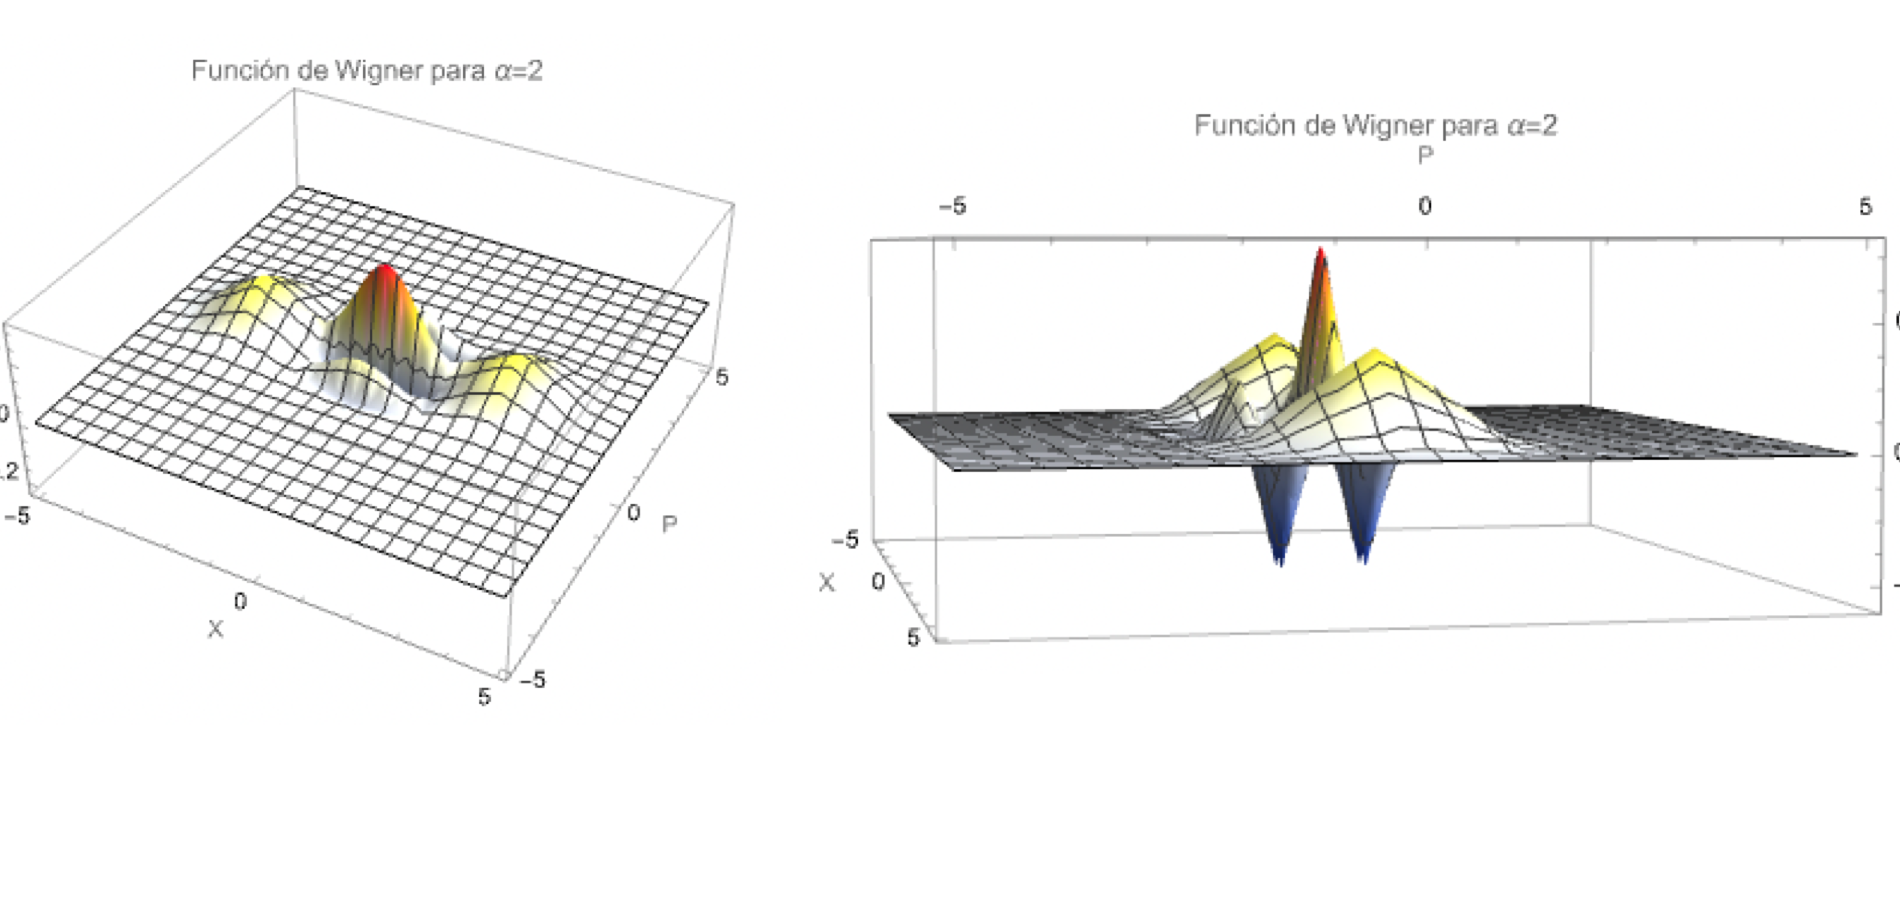
\includegraphics[width=0.96\linewidth]{../../notas-doctorado/imgs/wigner_gato_alpha2.png}
  \caption{Funci\'on de Wigner para una superposici\'on de estados coherentes con $\alpha=2$. Los dos picos corresponden a los estados coherentes separados y la regi\'on central muestra las franjas de interferencia.}
\end{figure}

\section{Ejercicios resueltos}

\subsection*{Ejercicio 1: producto interno entre posici\'on y momento}

Se considera el operador de traslaci\'on
\begin{equation}
  \hat \tau(\Delta)=\ee^{-\ii\hat p\Delta/\hbar},
\end{equation}
que transforma estados propios de posici\'on como
\begin{equation}
  \hat\tau(\Delta)\ket{x'}=\ket{x'+\Delta}.
\end{equation}
Para encontrar $\braket{x|p}$ se parte de la relaci\'on can\'onica
\begin{equation}
  [\hat x,\hat p]=\ii\hbar.
\end{equation}
Se proyecta entre $\bra{x}$ y $\ket{x'}$:
\begin{equation}
  \bra{x}[\hat x,\hat p]\ket{x'}
  =
  \ii\hbar\braket{x|x'}
  =
  \ii\hbar\delta(x-x').
\end{equation}
Pero el lado izquierdo tambi\'en es
\begin{align}
  \bra{x}\hat x\hat p\ket{x'}
  -
  \bra{x}\hat p\hat x\ket{x'}
  &=
  x\bra{x}\hat p\ket{x'}
  -
  x'\bra{x}\hat p\ket{x'}\\
  &=
  (x-x')\bra{x}\hat p\ket{x'}.
\end{align}
Entonces
\begin{equation}
  (x-x')\bra{x}\hat p\ket{x'}
  =
  \ii\hbar\delta(x-x').
\end{equation}
En el sentido distribucional, esto equivale a
\begin{equation}
  \bra{x}\hat p\ket{x'}=-\ii\hbar\,\delta'(x-x').
\end{equation}
Para un estado arbitrario $\ket\psi$,
\begin{align}
  \bra{x}\hat p\ket\psi
  &=
  \int_{-\infty}^{\infty}
  \bra{x}\hat p\ket{x'}\braket{x'|\psi}\,\dd x'\\
  &=
  -\ii\hbar
  \int_{-\infty}^{\infty}
  \delta'(x-x')\psi(x')\,\dd x'\\
  &=
  -\ii\hbar\frac{\dd\psi(x)}{\dd x}.
\end{align}
Por tanto,
\begin{equation}
  \boxed{\hat p\to -\ii\hbar\frac{\dd}{\dd x}}
\end{equation}
en la representaci\'on de posici\'on.

Si ahora $\ket p$ es eigenestado de momento,
\begin{equation}
  \hat p\ket p=p\ket p,
\end{equation}
entonces
\begin{equation}
  -\ii\hbar\frac{\dd}{\dd x}\braket{x|p}
  =
  p\braket{x|p}.
\end{equation}
Definiendo $u_p(x)=\braket{x|p}$,
\begin{equation}
  \frac{\dd u_p}{\dd x}
  =
  \frac{\ii p}{\hbar}u_p.
\end{equation}
La soluci\'on es
\begin{equation}
  u_p(x)=A\ee^{\ii px/\hbar}.
\end{equation}
La constante $A$ se fija con la normalizaci\'on delta:
\begin{align}
  \delta(p-p')
  &=
  \braket{p|p'}\\
  &=
  \int_{-\infty}^{\infty}
  \braket{p|x}\braket{x|p'}\,\dd x\\
  &=
  |A|^2
  \int_{-\infty}^{\infty}
  \ee^{\ii(p'-p)x/\hbar}\,\dd x\\
  &=
  |A|^2\,2\pi\hbar\,\delta(p-p').
\end{align}
As\'i,
\begin{equation}
  |A|^2=\frac{1}{2\pi\hbar}.
\end{equation}
Escogiendo $A$ real positiva,
\begin{equation}
  \boxed{
  \braket{x|p}
  =
  \frac{1}{\sqrt{2\pi\hbar}}\ee^{\ii px/\hbar}.
  }
\end{equation}
Esta expresi\'on lleva directamente a la transformada de Fourier entre
$\psi(x)$ y $\psi(p)$.

\subsection*{Ejercicio 2: construcci\'on de $\hat a$, $\adag$ y el estado base}

Se parte del hamiltoniano del oscilador arm\'onico,
\begin{equation}
  \hat H=\frac{\hat p^2}{2m}+\frac12m\omega^2\hat x^2.
\end{equation}
Se busca escribirlo como
\begin{equation}
  \hat H=E_0+\lambda\hat O^\dagger\hat O,
\end{equation}
con un operador lineal en $\hat x$ y $\hat p$. Se propone
\begin{equation}
  \hat O=c_x\hat x+\ii c_p\hat p,
  \qquad
  \hat O^\dagger=c_x\hat x-\ii c_p\hat p,
\end{equation}
donde $c_x$ y $c_p$ son reales. Entonces
\begin{align}
  \hat O^\dagger\hat O
  &=
  (c_x\hat x-\ii c_p\hat p)(c_x\hat x+\ii c_p\hat p)\\
  &=
  c_x^2\hat x^2+c_p^2\hat p^2
  +\ii c_xc_p\hat x\hat p
  -\ii c_xc_p\hat p\hat x\\
  &=
  c_x^2\hat x^2+c_p^2\hat p^2
  +\ii c_xc_p[\hat x,\hat p]\\
  &=
  c_x^2\hat x^2+c_p^2\hat p^2
  -c_xc_p\hbar.
\end{align}
Comparando $\lambda\hat O^\dagger\hat O+E_0$ con $\hat H$,
\begin{equation}
  \lambda c_x^2=\frac12m\omega^2,
  \qquad
  \lambda c_p^2=\frac{1}{2m},
  \qquad
  E_0=\lambda c_xc_p\hbar.
\end{equation}
La raz\'on entre las dos primeras ecuaciones da
\begin{equation}
  \frac{c_x}{c_p}=m\omega.
\end{equation}
Adem\'as,
\begin{equation}
  [\hat O,\hat O^\dagger]=2c_xc_p\hbar.
\end{equation}
Para que $\hat O^\dagger\hat O$ sea el operador de n\'umero se impone
\begin{equation}
  [\hat O,\hat O^\dagger]=1,
  \qquad
  2c_xc_p\hbar=1.
\end{equation}
Junto con $c_x/c_p=m\omega$,
\begin{equation}
  c_x=\sqrt{\frac{m\omega}{2\hbar}},
  \qquad
  c_p=\frac{1}{\sqrt{2m\omega\hbar}}.
\end{equation}
Por tanto,
\begin{equation}
  \hat a=\sqrt{\frac{m\omega}{2\hbar}}
  \left(\hat x+\frac{\ii}{m\omega}\hat p\right),
  \qquad
  \adag=\sqrt{\frac{m\omega}{2\hbar}}
  \left(\hat x-\frac{\ii}{m\omega}\hat p\right),
\end{equation}
y
\begin{equation}
  \hat H=\hbar\omega\left(\adag\hat a+\frac12\right).
\end{equation}

El estado base $\ket0$ satisface
\begin{equation}
  \hat a\ket0=0.
\end{equation}
En representaci\'on de posici\'on,
\begin{equation}
  \hat p=-\ii\hbar\frac{\dd}{\dd x}.
\end{equation}
Entonces
\begin{align}
  0
  &=
  \bra{x}\hat a\ket0\\
  &=
  \sqrt{\frac{m\omega}{2\hbar}}
  \left(
  x+\frac{\hbar}{m\omega}\frac{\dd}{\dd x}
  \right)\psi_0(x).
\end{align}
La ecuaci\'on diferencial es
\begin{equation}
  \frac{\dd\psi_0}{\dd x}
  =
  -\frac{m\omega}{\hbar}x\psi_0.
\end{equation}
Separando variables,
\begin{equation}
  \frac{\dd\psi_0}{\psi_0}
  =
  -\frac{m\omega}{\hbar}x\,\dd x.
\end{equation}
Integrando,
\begin{equation}
  \ln\psi_0
  =
  -\frac{m\omega}{2\hbar}x^2+C.
\end{equation}
Por tanto,
\begin{equation}
  \psi_0(x)=A\ee^{-m\omega x^2/(2\hbar)}.
\end{equation}
La normalizaci\'on exige
\begin{align}
  1
  &=
  \int_{-\infty}^{\infty}|\psi_0(x)|^2\,\dd x\\
  &=
  |A|^2
  \int_{-\infty}^{\infty}
  \ee^{-m\omega x^2/\hbar}\,\dd x\\
  &=
  |A|^2\sqrt{\frac{\pi\hbar}{m\omega}}.
\end{align}
Por tanto,
\begin{equation}
  |A|^2=\sqrt{\frac{m\omega}{\pi\hbar}},
  \qquad
  A=\left(\frac{m\omega}{\pi\hbar}\right)^{1/4}.
\end{equation}
Finalmente,
\begin{equation}
  \boxed{
  \psi_0(x)
  =
  \left(\frac{m\omega}{\pi\hbar}\right)^{1/4}
  \ee^{-m\omega x^2/(2\hbar)}.
  }
\end{equation}

\subsection*{Ejercicio 3: traslaci\'on espacial del vac\'io}

Se quiere calcular
\begin{equation}
  \bra{x}\ee^{-\ii\hat p\Delta/\hbar}\ket0.
\end{equation}
Como en representaci\'on de posici\'on
\begin{equation}
  \hat p=-\ii\hbar\frac{\dd}{\dd x},
\end{equation}
entonces
\begin{equation}
  \ee^{-\ii\hat p\Delta/\hbar}
  =
  \ee^{-\Delta\,\dd/\dd x}.
\end{equation}
La exponencial de una derivada act\'ua como operador de traslaci\'on:
\begin{equation}
  \ee^{-\Delta\,\dd/\dd x}f(x)=f(x-\Delta).
\end{equation}
Por tanto,
\begin{align}
  \bra{x}\ee^{-\ii\hat p\Delta/\hbar}\ket0
  &=
  \psi_0(x-\Delta)\\
  &=
  \left(\frac{m\omega}{\pi\hbar}\right)^{1/4}
  \exp\left[-\frac{m\omega}{2\hbar}(x-\Delta)^2\right].
\end{align}
La funci\'on de onda del vac\'io, centrada originalmente en $x=0$, queda
desplazada a $x=\Delta$.

La misma traslaci\'on puede escribirse como un desplazamiento coherente. Usando
\begin{equation}
  \hat p=\ii\sqrt{\frac{\hbar m\omega}{2}}(\adag-\hat a),
\end{equation}
se obtiene
\begin{align}
  \ee^{-\ii\hat p\Delta/\hbar}
  &=
  \exp\left[
  \Delta\sqrt{\frac{m\omega}{2\hbar}}(\adag-\hat a)
  \right]\\
  &=
  \hat D(\alpha_\Delta),
\end{align}
con
\begin{equation}
  \alpha_\Delta=\Delta\sqrt{\frac{m\omega}{2\hbar}}\in\mathbb R.
\end{equation}
Por tanto,
\begin{equation}
  \ee^{-\ii\hat p\Delta/\hbar}\ket0
  =
  \ket{\alpha_\Delta}.
\end{equation}
Un desplazamiento espacial del vac\'io es un estado coherente con $\alpha$ real.

\subsection*{Ejercicio 4: forma normal y desplazamiento del estado coherente}

Se considera el estado
\begin{equation}
  \ket{\beta}
  =
  \ee^{-|\beta|^2/2}
  \sum_{n=0}^{\infty}\frac{\beta^n}{\sqrt{n!}}\ket n,
  \qquad \beta\in\mathbb C.
\end{equation}
Primero se verifica que es eigenestado de $\hat a$. Aplicando $\hat a$,
\begin{align}
  \hat a\ket{\beta}
  &=
  \ee^{-|\beta|^2/2}
  \sum_{n=1}^{\infty}
  \frac{\beta^n}{\sqrt{n!}}\sqrt n\,\ket{n-1}.
\end{align}
Se cambia $m=n-1$:
\begin{align}
  \hat a\ket{\beta}
  &=
  \ee^{-|\beta|^2/2}
  \sum_{m=0}^{\infty}
  \frac{\beta^{m+1}}{\sqrt{(m+1)!}}\sqrt{m+1}\,\ket m\\
  &=
  \beta\,
  \ee^{-|\beta|^2/2}
  \sum_{m=0}^{\infty}
  \frac{\beta^m}{\sqrt{m!}}\ket m\\
  &=
  \beta\ket\beta.
\end{align}

Ahora se prueba que
\begin{equation}
  \ket{\beta}
  =
  \ee^{-|\beta|^2/2}\ee^{\beta\adag}\ket0.
\end{equation}
En efecto,
\begin{align}
  \ee^{\beta\adag}\ket0
  &=
  \sum_{k=0}^{\infty}
  \frac{\beta^k}{k!}(\adag)^k\ket0\\
  &=
  \sum_{k=0}^{\infty}
  \frac{\beta^k}{k!}\sqrt{k!}\ket k\\
  &=
  \sum_{k=0}^{\infty}
  \frac{\beta^k}{\sqrt{k!}}\ket k.
\end{align}
Multiplicando por $\ee^{-|\beta|^2/2}$ se recupera $\ket\beta$.

Adem\'as,
\begin{equation}
  \ee^{-\beta^*\hat a}\ket0=\ket0,
\end{equation}
porque todas las potencias positivas de $\hat a$ aniquilan el vac\'io. Por
eso,
\begin{equation}
  \ket\beta
  =
  \ee^{-|\beta|^2/2}
  \ee^{\beta\adag}
  \ee^{-\beta^*\hat a}\ket0.
\end{equation}
Usando Baker-Campbell-Hausdorff,
\begin{equation}
  \ee^{\beta\adag}\ee^{-\beta^*\hat a}
  =
  \ee^{\beta\adag-\beta^*\hat a+|\beta|^2/2},
\end{equation}
pues
\begin{equation}
  [\beta\adag,-\beta^*\hat a]=|\beta|^2.
\end{equation}
Entonces
\begin{equation}
  \ee^{-|\beta|^2/2}
  \ee^{\beta\adag}
  \ee^{-\beta^*\hat a}
  =
  \ee^{\beta\adag-\beta^*\hat a}
  =
  \hat D(\beta).
\end{equation}
Por tanto,
\begin{equation}
  \boxed{\ket\beta=\hat D(\beta)\ket0.}
\end{equation}

\subsection*{Ejercicio 5: impulso de momento sobre el vac\'io}

Se estudia el estado
\begin{equation}
  \ee^{-\ii\hat p x_0/\hbar}\ket0.
\end{equation}
Usando de nuevo
\begin{equation}
  \hat p=\ii\sqrt{\frac{\hbar m\omega}{2}}(\adag-\hat a),
\end{equation}
se tiene
\begin{align}
  \ee^{-\ii\hat p x_0/\hbar}\ket0
  &=
  \exp\left[
  x_0\sqrt{\frac{m\omega}{2\hbar}}(\adag-\hat a)
  \right]\ket0\\
  &=
  \hat D(\beta)\ket0,
\end{align}
donde
\begin{equation}
  \boxed{
  \beta=x_0\sqrt{\frac{m\omega}{2\hbar}}.
  }
\end{equation}
Como $\beta$ es real, el desplazamiento es en la cuadratura de posici\'on. Por
lo tanto,
\begin{equation}
  \ee^{-\ii\hat p x_0/\hbar}\ket0=\ket\beta.
\end{equation}

La evoluci\'on temporal bajo el oscilador arm\'onico es entonces inmediata:
\begin{equation}
  \ket{\psi(t)}
  =
  \ee^{-\ii\hat Ht/\hbar}\ket\beta
  =
  \ee^{-\ii\omega t/2}\ket{\beta\ee^{-\ii\omega t}}.
\end{equation}
La fase global $\ee^{-\ii\omega t/2}$ no cambia observables. El centro del
estado gira en espacio fase:
\begin{equation}
  \beta(t)=\beta\ee^{-\ii\omega t}.
\end{equation}
Por eso un desplazamiento inicial puramente espacial se convierte, con el
tiempo, en una combinaci\'on de desplazamiento en posici\'on y momento, como
ocurre en la evoluci\'on cl\'asica del oscilador arm\'onico.

\end{document}
